\section{Introduction (Lec. 1)}
\subsection{The Well-specified Case}
Given a collection of $n$ samples $\{x_i\}_{i=1}^n$ sampled from a fixed distribution $\mathbb{P}$. Let $f^*$ be the ``true'' estimator that minimizes some loss $\ell(x; f)$, i.e., $f^* := \arg \min_{f\in\mathcal{F}} \mathbb{E}_x\ell(x_i; f)$. 

\begin{definition}[Risk] The estimation of losses is called \textit{risk}:
\begin{itemize}
\setlength\itemsep{-0.5em}
    \item Empirical risk: $$R_n(f) := \frac{1}{n} \sum_{i=1}^n \ell(x_i; f)$$
    \item Population risk: $$R(f) := \mathbb{E}_{x \sim \mathbb{P}} \ell(x; f)$$
\end{itemize}
\end{definition}
\textbf{Remark}: Please note that the notation in our course is slightly different from the MW Chapter 4, where it uses a more burdensome notation as $R(f, f^*)$. Here, the $f^*$ is omitted since it is fixed in a problem.
\begin{definition}[Excess risk]
The excess risk is defined as $$\mathcal{E}_n(\hat{f}_n, f^*) := R(\hat{f}_n) - R(f^*).$$
\end{definition}

\begin{theorem}[Risk decomposition]
The excess risk $R(\hat{f}) - R(f^*)$ can be decomposed into
\begin{align*} = \underbrace{R(\hat{f}) - R_n(\hat{f})}_{T_1} + \underbrace{ R_n(\hat{f}) - R_n(f^*)}_{T_3} + \underbrace{R_n(f^*) - R(f^*)}_{T_2}
\end{align*}
\end{theorem}
\textbf{Remark}: The following figure illustrate the risk decomposition. In the figure, the upper and lower layers represent the empirical risk and the population risk, respectively.
\begin{center}
    \tikzset{every picture/.style={line width=0.75pt}} %set default line width to 0.75pt        
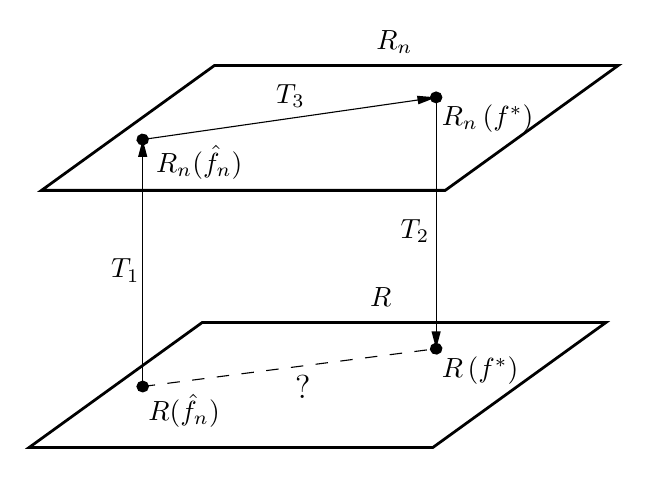
\begin{tikzpicture}[x=0.75pt,y=0.75pt,yscale=-0.7,xscale=0.75]
%uncomment if require: \path (0,503); %set diagram left start at 0, and has height of 503

%Shape: Parallelogram [id:dp6379841658274947] 
\draw  [line width=1]  (250.15,328) -- (509.5,328) -- (398.35,414) -- (139,414) -- cycle ;
%Shape: Parallelogram [id:dp5659534429170581] 
\draw  [line width=1]  (258.15,151) -- (517.5,151) -- (406.35,237) -- (147,237) -- cycle ;
%Straight Lines [id:da458543701942727] 
\draw    (212,372) -- (212,204) ;
\draw [shift={(212,202)}, rotate = 450] [fill={rgb, 255:red, 0; green, 0; blue, 0 }  ][line width=0.08]  [draw opacity=0] (12,-3) -- (0,0) -- (12,3) -- cycle    ;
\draw [shift={(212,372)}, rotate = 270] [color={rgb, 255:red, 0; green, 0; blue, 0 }  ][fill={rgb, 255:red, 0; green, 0; blue, 0 }  ][line width=0.75]      (0, 0) circle [x radius= 3.35, y radius= 3.35]   ;
%Straight Lines [id:da6580046139798694] 
\draw    (212,202) -- (398.52,173.3) ;
\draw [shift={(400.5,173)}, rotate = 531.25] [fill={rgb, 255:red, 0; green, 0; blue, 0 }  ][line width=0.08]  [draw opacity=0] (12,-3) -- (0,0) -- (12,3) -- cycle    ;
\draw [shift={(212,202)}, rotate = 351.25] [color={rgb, 255:red, 0; green, 0; blue, 0 }  ][fill={rgb, 255:red, 0; green, 0; blue, 0 }  ][line width=0.75]      (0, 0) circle [x radius= 3.35, y radius= 3.35]   ;
%Straight Lines [id:da5733317875250146] 
\draw    (400.5,173) -- (400.5,344) ;
\draw [shift={(400.5,346)}, rotate = 270] [fill={rgb, 255:red, 0; green, 0; blue, 0 }  ][line width=0.08]  [draw opacity=0] (12,-3) -- (0,0) -- (12,3) -- cycle    ;
\draw [shift={(400.5,173)}, rotate = 90] [color={rgb, 255:red, 0; green, 0; blue, 0 }  ][fill={rgb, 255:red, 0; green, 0; blue, 0 }  ][line width=0.75]      (0, 0) circle [x radius= 3.35, y radius= 3.35]   ;
%Straight Lines [id:da12727382381339924] 
\draw  [dash pattern={on 4.5pt off 4.5pt}]  (212,372) -- (400.5,346) ;
\draw [shift={(400.5,346)}, rotate = 352.15] [color={rgb, 255:red, 0; green, 0; blue, 0 }  ][fill={rgb, 255:red, 0; green, 0; blue, 0 }  ][line width=0.75]      (0, 0) circle [x radius= 3.35, y radius= 3.35]   ;

% Text Node
\draw (360.35,125.4) node [anchor=north west][inner sep=0.75pt]    {$R_{n}$};
% Text Node
\draw (356.35,302.4) node [anchor=north west][inner sep=0.75pt]    {$R$};
% Text Node
\draw (214,375.4) node [anchor=north west][inner sep=0.75pt]    {$R(\hat{f}_{n})$};
% Text Node
\draw (219,204.4) node [anchor=north west][inner sep=0.75pt]    {$R_{n}(\hat{f}_{n})$};
% Text Node
\draw (402.5,176.4) node [anchor=north west][inner sep=0.75pt]    {$R_{n}\left( f^{*}\right)$};
% Text Node
\draw (402.5,349.4) node [anchor=north west][inner sep=0.75pt]    {$R\left( f^{*}\right)$};
% Text Node
\draw (308.25,362.4) node [anchor=north west][inner sep=0.75pt]  [font=\large]  {$?$};
\draw (190,282.4) node [anchor=north west][inner sep=0.75pt]    {$T_{1}$};
% Text Node
\draw (376,255.4) node [anchor=north west][inner sep=0.75pt]    {$T_{2}$};
% Text Node
\draw (296,162.4) node [anchor=north west][inner sep=0.75pt]    {$T_{3}$};
\end{tikzpicture}
\vspace{1em}

\caption{\textbf{Figure}: Risk decomposition (well-specified)}
\end{center}

\subsection{The Mis-specification Case}
We call the problem mis-specification, when $f^* \not\in \mathcal{F}$.
\begin{theorem}[Bias-variance trade-off]
The excess risk $R(\hat{f}) - R(f^*)$ can be decomposed into 
\begin{align*} 
R(\widehat{f}_{n})-R\left(f^{\star}\right)=\underbrace{R(\widehat{f}_{n})-R\left(f^{\star, \mathcal{F}}\right)}_{\text {"Variance" }}+\underbrace{R\left(f^{\star, \mathcal{F}}\right)-R\left(f^{\star}\right)}_{\text {"Bias" }=\text { "approx error" }}
\end{align*}
where $f^{\star, \mathcal{F}} = \arg\min_{f\in\mathcal{F}} R(f)$.
\end{theorem}
\textbf{Remark}: The following figure provides some insights.
\begin{center}
    \tikzset{every picture/.style={line width=0.75pt}} %set default line width to 0.75pt        

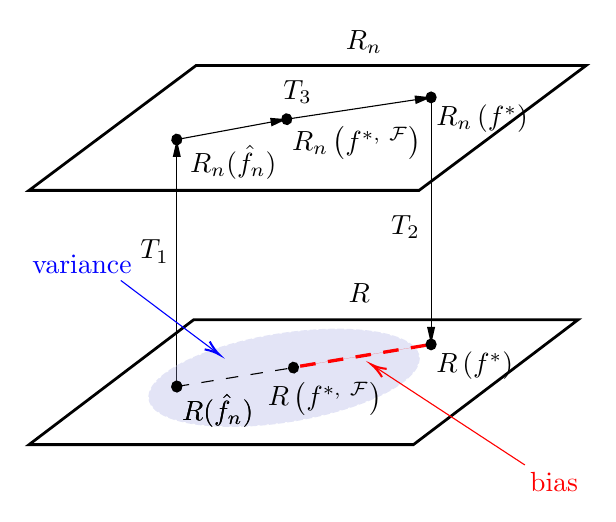
\begin{tikzpicture}[x=0.75pt,y=0.75pt,yscale=-0.7,xscale=0.65]
%uncomment if require: \path (0,428); %set diagram left start at 0, and has height of 428

%Shape: Parallelogram [id:dp7274687411777527] 
\draw  [line width=1]  (211.6,259) -- (496.5,259) -- (374.4,345) -- (89.5,345) -- cycle ;
%Shape: Parallelogram [id:dp5477732282695964] 
\draw  [line width=1]  (213.4,84) -- (502.5,84) -- (378.6,170) -- (89.5,170) -- cycle ;
%Straight Lines [id:da2018530395235334] 
\draw    (199,305) -- (199,137) ;
\draw [shift={(199,135)}, rotate = 450] [fill={rgb, 255:red, 0; green, 0; blue, 0 }  ][line width=0.08]  [draw opacity=0] (12,-3) -- (0,0) -- (12,3) -- cycle    ;
\draw [shift={(199,305)}, rotate = 270] [color={rgb, 255:red, 0; green, 0; blue, 0 }  ][fill={rgb, 255:red, 0; green, 0; blue, 0 }  ][line width=0.75]      (0, 0) circle [x radius= 3.35, y radius= 3.35]   ;
%Straight Lines [id:da7590655674070557] 
\draw    (199,135) -- (278.53,121.34) ;
\draw [shift={(280.5,121)}, rotate = 530.25] [fill={rgb, 255:red, 0; green, 0; blue, 0 }  ][line width=0.08]  [draw opacity=0] (12,-3) -- (0,0) -- (12,3) -- cycle    ;
\draw [shift={(199,135)}, rotate = 350.25] [color={rgb, 255:red, 0; green, 0; blue, 0 }  ][fill={rgb, 255:red, 0; green, 0; blue, 0 }  ][line width=0.75]      (0, 0) circle [x radius= 3.35, y radius= 3.35]   ;
%Straight Lines [id:da94095897726301] 
\draw    (387.5,106) -- (387.5,274) ;
\draw [shift={(387.5,276)}, rotate = 270] [fill={rgb, 255:red, 0; green, 0; blue, 0 }  ][line width=0.08]  [draw opacity=0] (12,-3) -- (0,0) -- (12,3) -- cycle    ;
\draw [shift={(387.5,106)}, rotate = 90] [color={rgb, 255:red, 0; green, 0; blue, 0 }  ][fill={rgb, 255:red, 0; green, 0; blue, 0 }  ][line width=0.75]      (0, 0) circle [x radius= 3.35, y radius= 3.35]   ;
%Straight Lines [id:da1976293015627566] 
\draw    (280.5,121) -- (385.52,106.28) ;
\draw [shift={(387.5,106)}, rotate = 532.02] [fill={rgb, 255:red, 0; green, 0; blue, 0 }  ][line width=0.08]  [draw opacity=0] (12,-3) -- (0,0) -- (12,3) -- cycle    ;
\draw [shift={(280.5,121)}, rotate = 352.02] [color={rgb, 255:red, 0; green, 0; blue, 0 }  ][fill={rgb, 255:red, 0; green, 0; blue, 0 }  ][line width=0.75]      (0, 0) circle [x radius= 3.35, y radius= 3.35]   ;
%Shape: Ellipse [id:dp35271263746573145] 
\draw  [color={rgb, 255:red, 255; green, 255; blue, 255 }  ,draw opacity=1 ][fill={rgb, 255:red, 152; green, 157; blue, 223 }  ,fill opacity=0.27 ][dash pattern={on 0.84pt off 2.51pt}] (185.95,299) .. controls (207.74,280.32) and (266.84,265.18) .. (317.95,265.18) .. controls (369.06,265.18) and (392.84,280.32) .. (371.05,299) .. controls (349.26,317.68) and (290.16,332.82) .. (239.05,332.82) .. controls (187.94,332.82) and (164.16,317.68) .. (185.95,299) -- cycle ;
%Straight Lines [id:da7033382741571668] 
\draw  [dash pattern={on 4.5pt off 4.5pt}]  (199,305) -- (285.5,292) ;
\draw [shift={(285.5,292)}, rotate = 351.45] [color={rgb, 255:red, 0; green, 0; blue, 0 }  ][fill={rgb, 255:red, 0; green, 0; blue, 0 }  ][line width=0.75]      (0, 0) circle [x radius= 3.35, y radius= 3.35]   ;
\draw [shift={(199,305)}, rotate = 351.45] [color={rgb, 255:red, 0; green, 0; blue, 0 }  ][fill={rgb, 255:red, 0; green, 0; blue, 0 }  ][line width=0.75]      (0, 0) circle [x radius= 3.35, y radius= 3.35]   ;
%Straight Lines [id:da46898574266560433] 
\draw [color={rgb, 255:red, 255; green, 0; blue, 0 }  ,draw opacity=1 ][fill={rgb, 255:red, 255; green, 0; blue, 0 }  ,fill opacity=1 ][line width=1.2]  [dash pattern={on 5.63pt off 4.5pt}]  (290.5,291) -- (387.5,276) ;
%Straight Lines [id:da534934643638076] 
\draw    (387.5,276) ;
\draw [shift={(387.5,276)}, rotate = 0] [color={rgb, 255:red, 0; green, 0; blue, 0 }  ][fill={rgb, 255:red, 0; green, 0; blue, 0 }  ][line width=0.75]      (0, 0) circle [x radius= 3.35, y radius= 3.35]   ;
%Straight Lines [id:da8410108610917204] 
\draw [color={rgb, 255:red, 255; green, 0; blue, 0 }  ,draw opacity=1 ]   (457,359) -- (345.21,291.04) ;
\draw [shift={(343.5,290)}, rotate = 391.3] [color={rgb, 255:red, 255; green, 0; blue, 0 }  ,draw opacity=1 ][line width=0.75]    (10.93,-3.29) .. controls (6.95,-1.4) and (3.31,-0.3) .. (0,0) .. controls (3.31,0.3) and (6.95,1.4) .. (10.93,3.29)   ;
%Straight Lines [id:da6689238100303159] 
\draw [color={rgb, 255:red, 0; green, 0; blue, 255 }  ,draw opacity=1 ]   (157.5,232) -- (228.86,281.85) ;
\draw [shift={(230.5,283)}, rotate = 214.94] [color={rgb, 255:red, 0; green, 0; blue, 255 }  ,draw opacity=1 ][line width=0.75]    (10.93,-3.29) .. controls (6.95,-1.4) and (3.31,-0.3) .. (0,0) .. controls (3.31,0.3) and (6.95,1.4) .. (10.93,3.29)   ;

% Text Node
\draw (322.35,58.4) node [anchor=north west][inner sep=0.75pt]    {$R_{n}$};
% Text Node
\draw (324.35,232.4) node [anchor=north west][inner sep=0.75pt]    {$R$};
% Text Node
\draw (201,308.4) node [anchor=north west][inner sep=0.75pt]    {$R(\hat{f}_{n})$};
% Text Node
\draw (207,137.4) node [anchor=north west][inner sep=0.75pt]    {$R_{n}(\hat{f}_{n})$};
% Text Node
\draw (389.5,109.4) node [anchor=north west][inner sep=0.75pt]    {$R_{n}\left( f^{*}\right)$};
% Text Node
\draw (389.5,279.4) node [anchor=north west][inner sep=0.75pt]    {$R\left( f^{*}\right)$};
% Text Node
\draw (282.5,124.4) node [anchor=north west][inner sep=0.75pt]    {$R_{n}\left( f^{*,\ \mathcal{F}}\right)$};
% Text Node
\draw (264.5,300.4) node [anchor=north west][inner sep=0.75pt]    {$R\left( f^{*,\ \mathcal{F}}\right)$};
\draw (170,202.4) node [anchor=north west][inner sep=0.75pt]    {$T_{1}$};
% Text Node
\draw (356,185.4) node [anchor=north west][inner sep=0.75pt]    {$T_{2}$};
% Text Node
\draw (276,92.4) node [anchor=north west][inner sep=0.75pt]    {$T_{3}$};
% Text Node
\draw (459,362.4) node [anchor=north west][inner sep=0.75pt]  [color=red  ,opacity=1 ]  {$\color{red} \mathrm{bias}$};
% Text Node
\draw (201,308.4) node [anchor=north west][inner sep=0.75pt]    {$R(\hat{f}_{n})$};
% Text Node
\draw (90,212.4) node [anchor=north west][inner sep=0.75pt]  [color=blue  ,opacity=1 ]  {$\color{blue} \mathrm{variance}$};
\end{tikzpicture}

\caption{\textbf{Figure}: Bias and variance under mis-specification}
\end{center}

